\begin{frame}
  %\begin{figure}
  %  \centering
  %  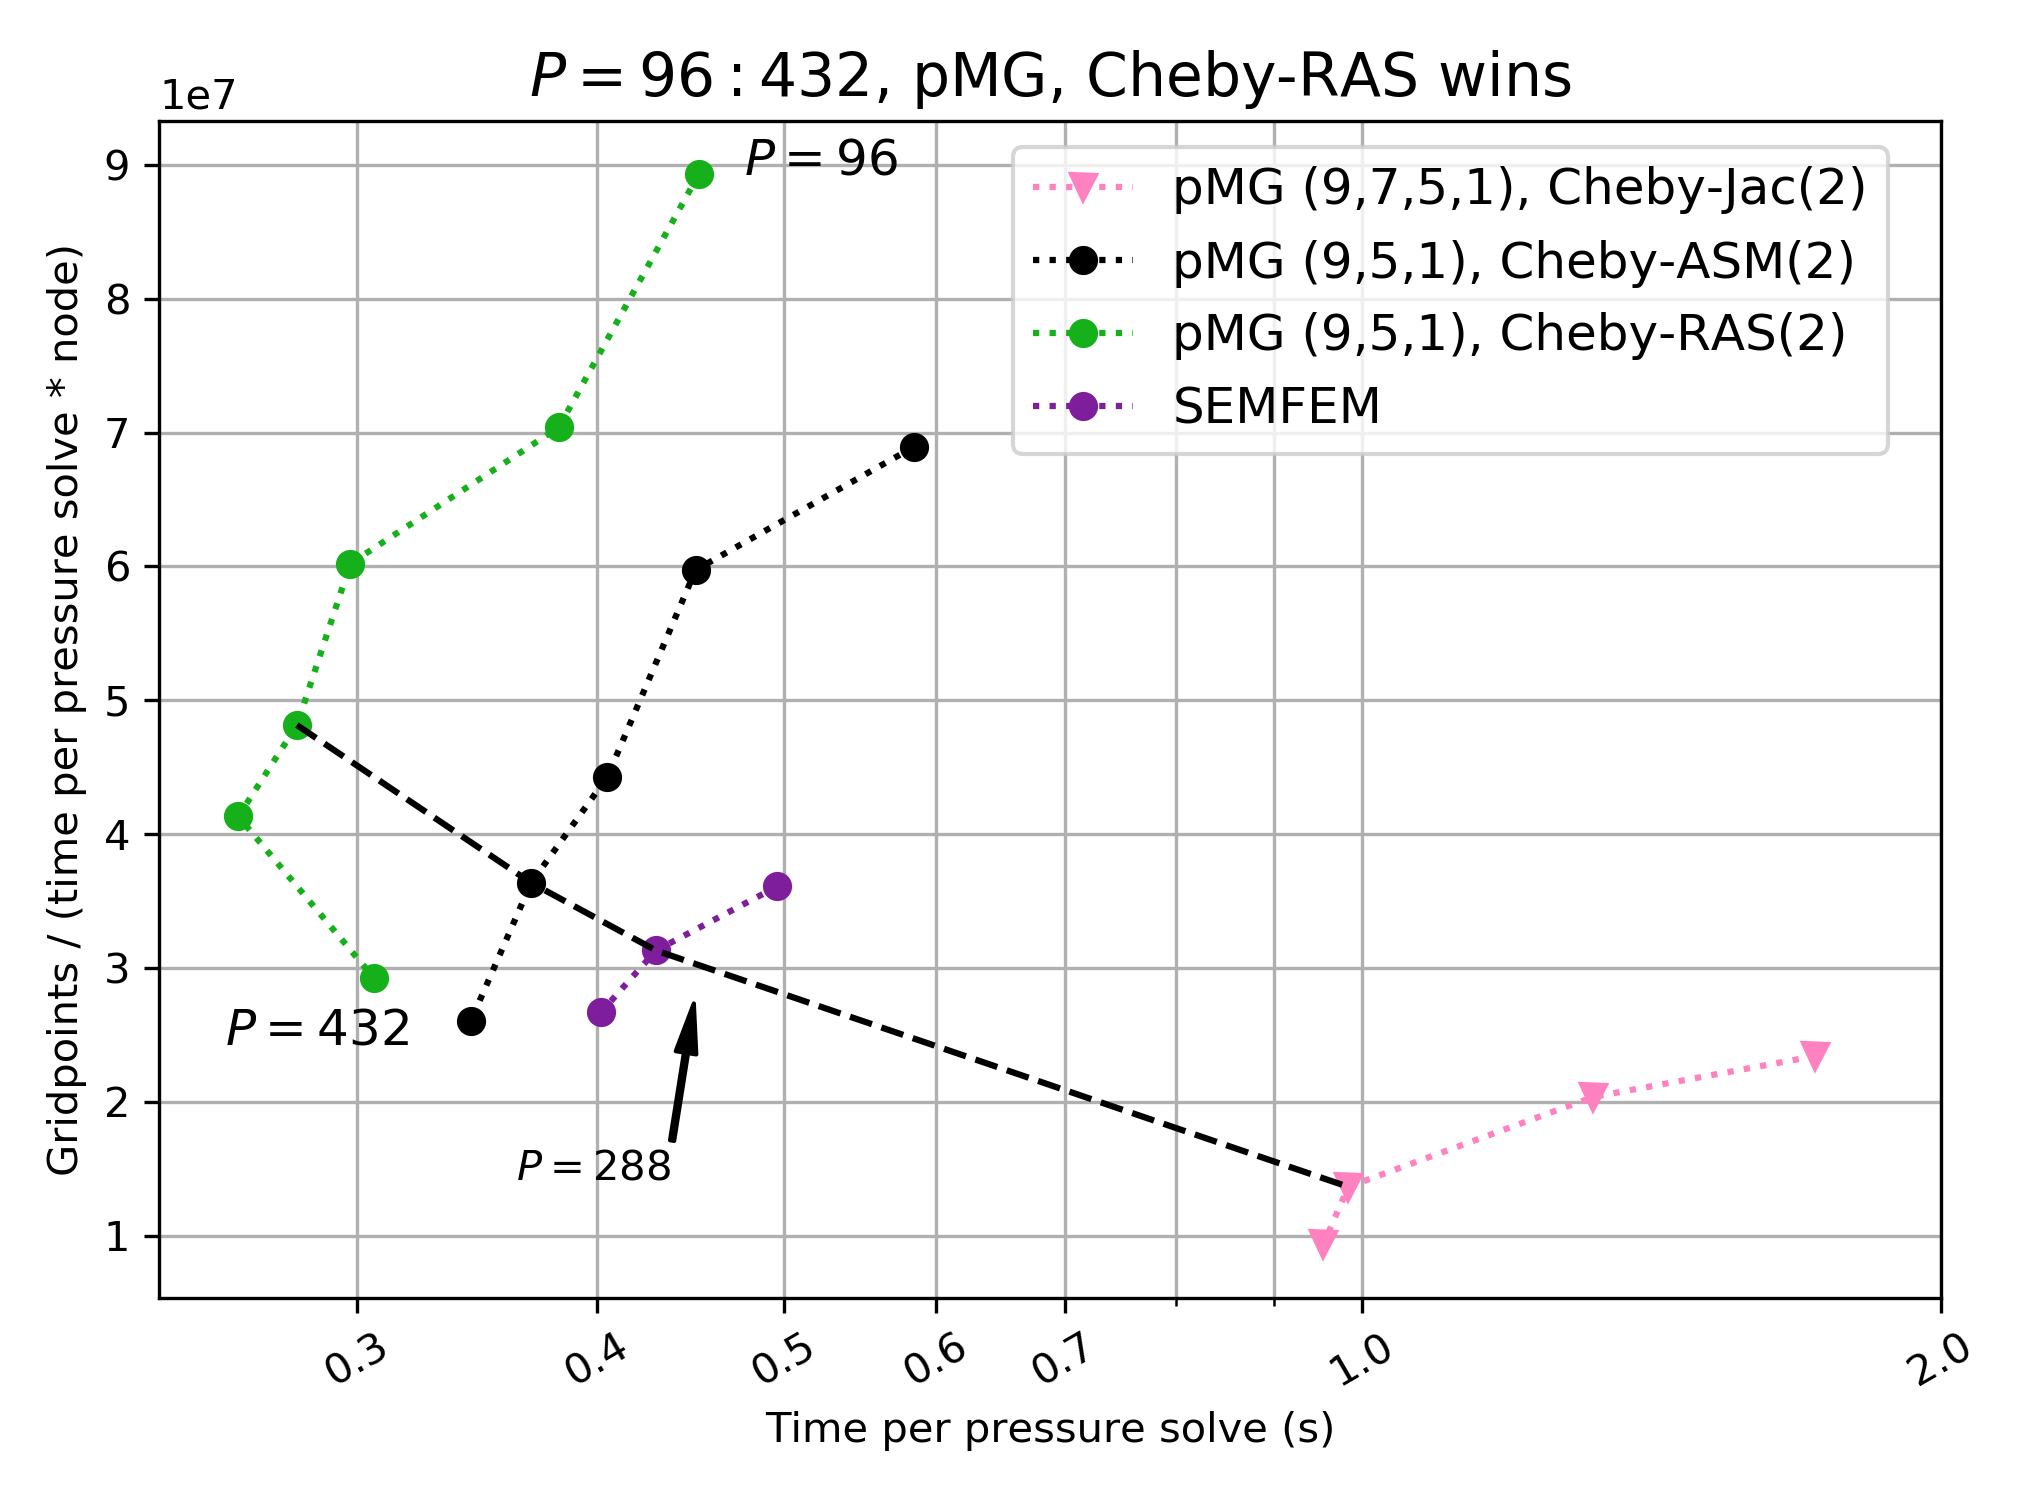
\includegraphics[width=\textwidth]{../figs/bsb-scaling.png}
  
  %  \vspace{-0.35cm}
  %  \captionsetup{labelformat=empty}
  %  \caption{
  %    \small
  %    Strong scaling results on Summit for the Boeing speed bump problem.
  %  }
  %  \label{fig:scaling-study-bsb}
  
  %\end{figure}
  \begin{figure}
    {\setlength{\unitlength}{\textwidth}
      \begin{picture}(1,0.75)(0,0)
        \put(0.0,0.0){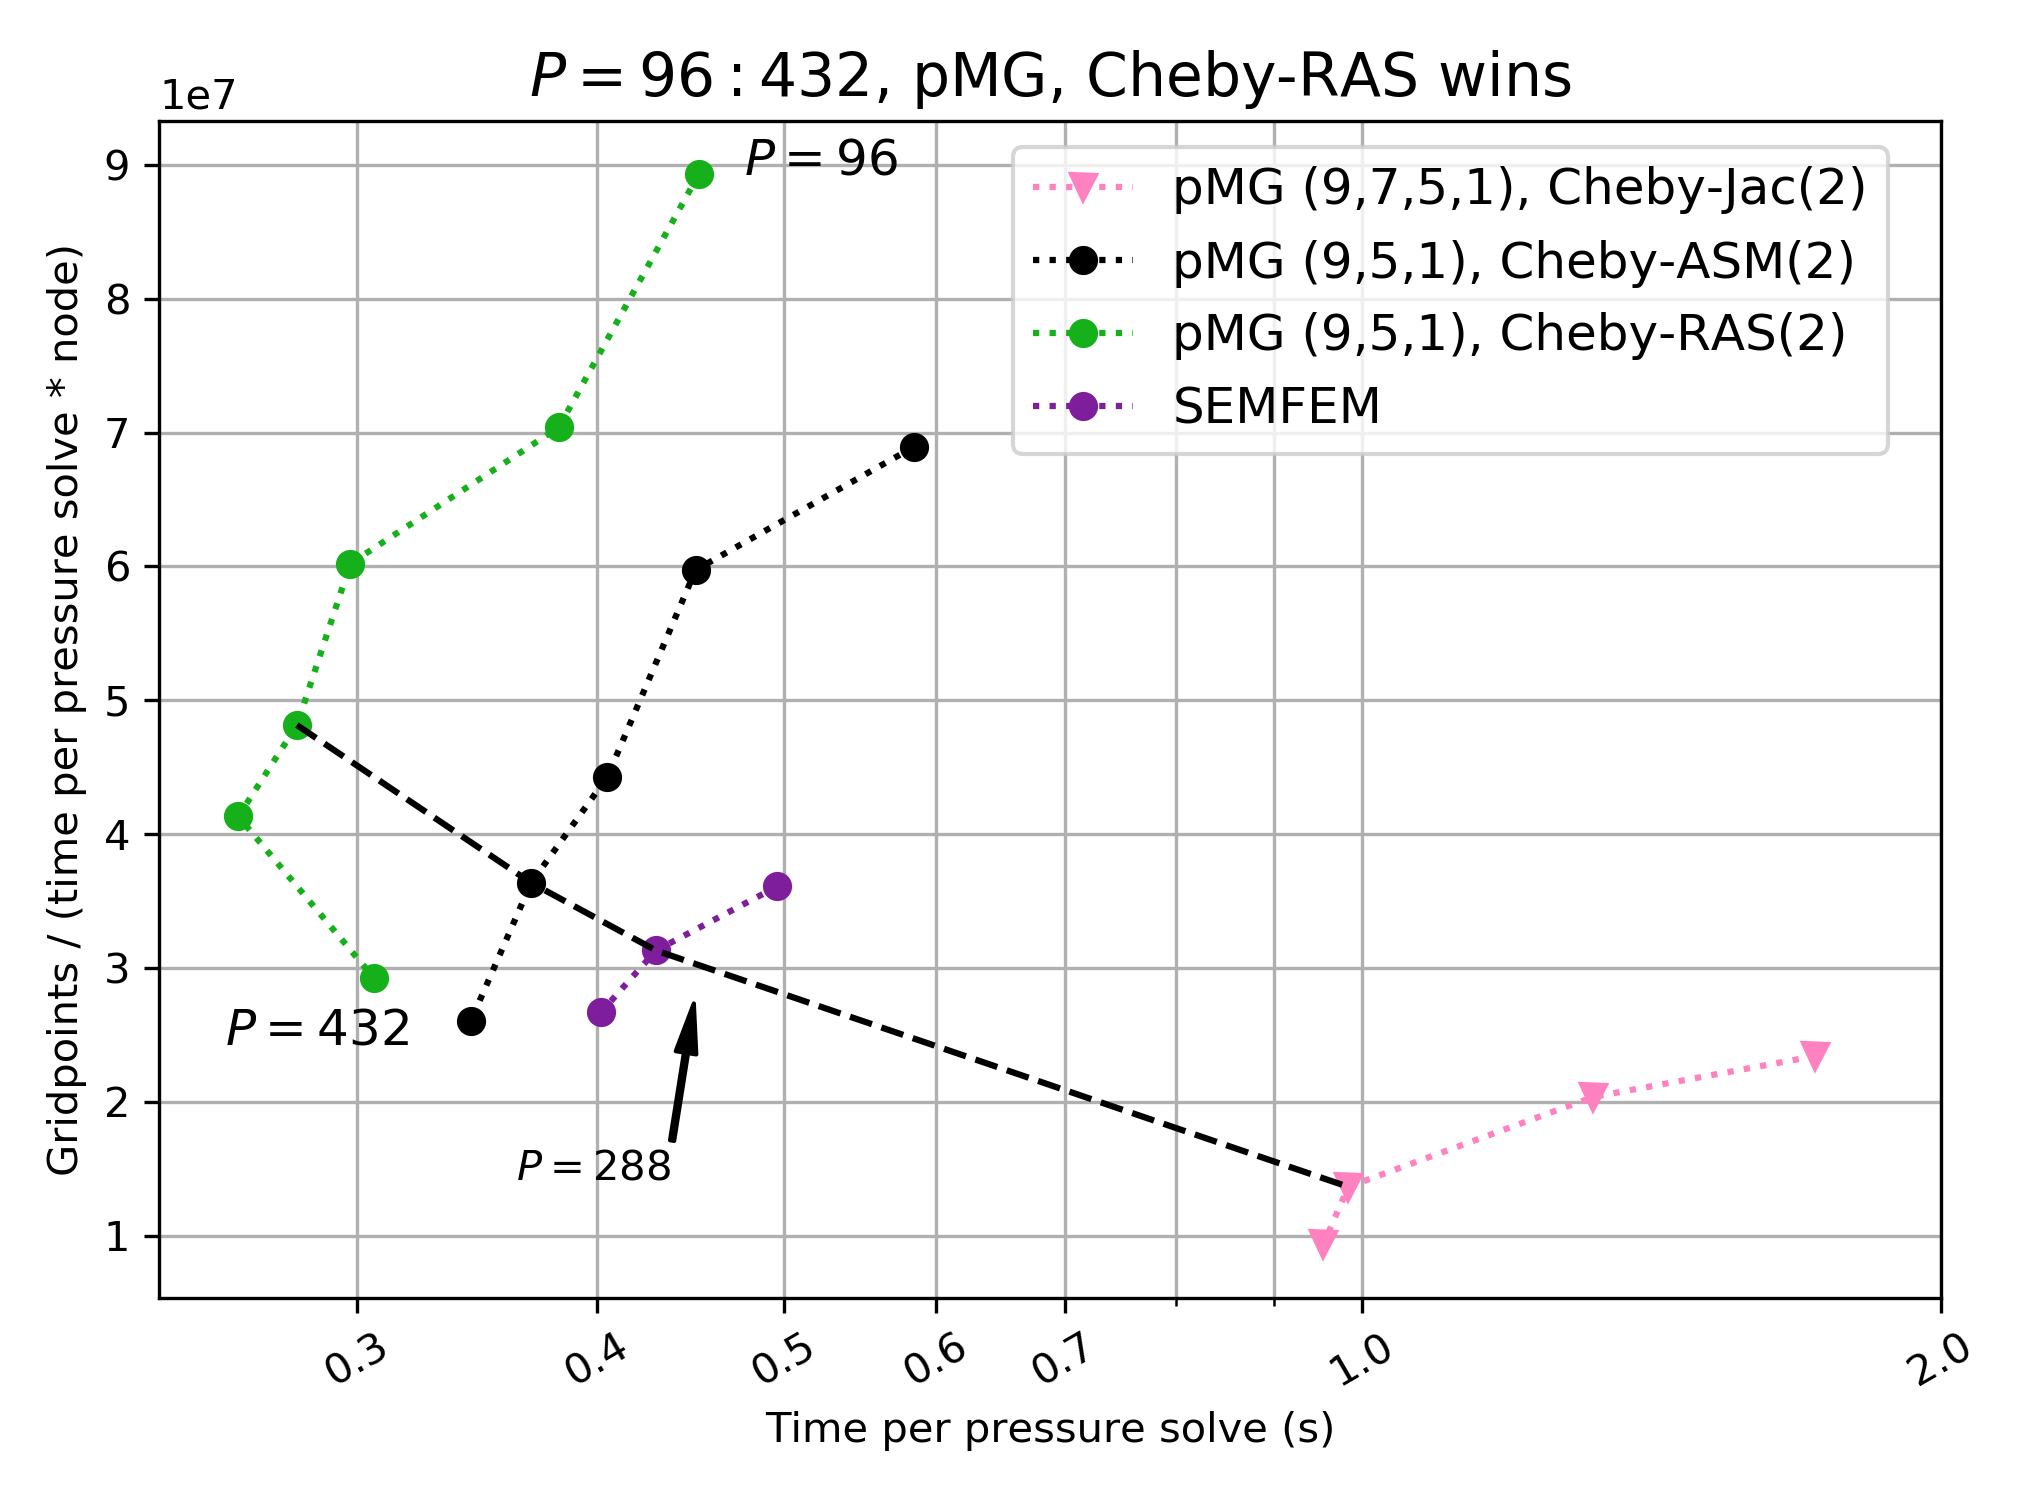
\includegraphics[width=\textwidth]{../figs/bsb-scaling.png}}
        \put(0.6,0.35){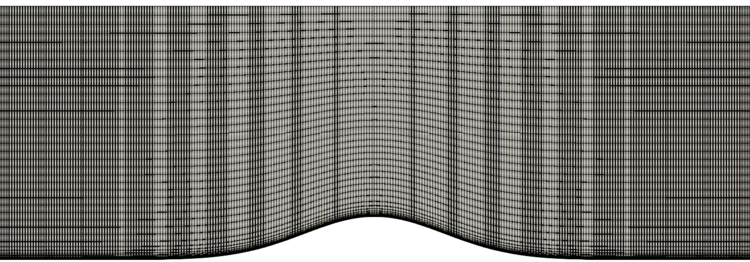
\includegraphics[width=0.3\textwidth]{../figs/BoeingSpeedBump.png}}
      \end{picture}}
    \captionsetup{labelformat=empty}
    \caption{
      \small
      Strong scaling results on Summit for the Boeing speed bump problem.
    }
  \end{figure}
\end{frame}